\documentclass[a4paper,11pt,notitlepage,halfparskip,headsepline,normalheadings,twoside]{scrartcl}
\usepackage{fontenc}
\usepackage{scrpage2}
\usepackage[german]{babel}
\usepackage[utf8x]{inputenc}
%\usepackage{keystroke}
\usepackage{pstricks}
\newlength{\tikey}
\newcommand{\keystroke}[1]{\settowidth{\tikey}{\scriptsize #1}\psframebox[framearc=0.2]{\parbox{\tikey}{\scriptsize\textsf{#1}}}}
\usepackage{graphicx}
\usepackage{multicol}
%\usepackage{draftcopy}
\usepackage{picinpar}
\usepackage{amssymb}
\usepackage{wasysym}
\usepackage{booktabs}
\usepackage{longtable}
%\usepackage{url}
\usepackage[pdfauthor={Mathias Weyland},pdftitle={Stochastik mit dem TI-Taschenrechner},pdfstartview=FitH,pdfborder={0 0 0}]{hyperref}
\usepackage{breakurl}
\usepackage{titlesec}
\titlespacing{\section}{0pt}{*0}{*0}
%\usepackage{setspace}
%\addtolength{\textheight}{3mm}
%\onehalfspacing
\sloppy
\setkomafont{pagehead}{\normalfont\normalcolor}
\renewcommand*{\titlepagestyle}{empty}

\title{Stochastik mit dem TI-Taschenrechner}
\date{Version 2.1}
\author{Mathias Weyland}
\pagestyle{headings}
%\ohead{Schreibwerkstatt, WS 06/07}
%\ihead{31. Januar 2007}
%\rfoot{}
%\ofoot{\pagemark}

\begin{document}
\maketitle

\begin{center}
\begin{multicols}{2}
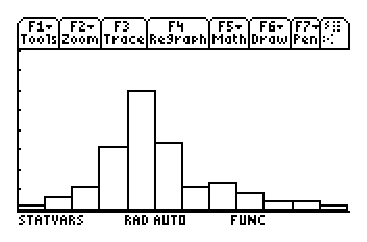
\includegraphics{eps/titlepage1}
\columnbreak
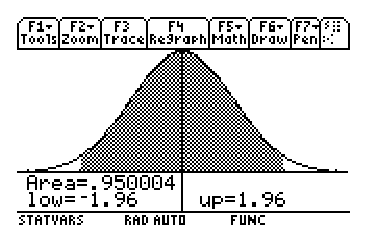
\includegraphics{eps/titlepage2}
\end{multicols}
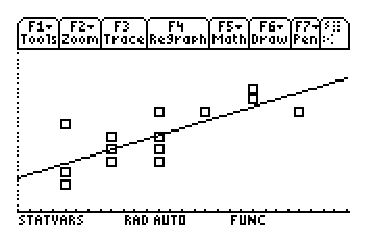
\includegraphics{eps/titlepage3}
\end{center}
\newpage
\section{Vorwort}
Dieses Skript beschreibt den sinnvollen Umgang mit den Taschenrechner TI-89,
TI-89 Titanium, TI-92 Plus und TI-Voyage\texttrademark~200 der Firma Texas
Instruments. Sowohl Screenshots als auch Anweisungen wurden mit Hilfe eines
TI-89 mit OS-Version 2.09 erstellt, unterscheiden sich aber von anderen Modellen
und OS-Versionen nur unmassgeblich. Sämtliche Taschenrechner-Funktionen sind auf
Englisch angegeben.

Im ersten Teil werden nützliche Tricks und Funktionen allgemein und mit Fokus
auf Stochastik vermittelt, während sich der zweite Teil in die Arbeit mit dem
\textit{Stats/List Editor}, einer Software, welche von Texas Instruments
entwickelt und kostenlos zu Verfügung gestellt wird, vertieft. Der
\textit{Stats/List Editor} wird im zweiten Teil nach der Installationshilfe
(Abschnitt \ref{installation}) vorausgesetzt.

\newpage


\tableofcontents
\newpage

\part{Allgemeine Handhabung}

\section{Fakultät und Binomialkoeffizent}
\begin{window}[0,l,{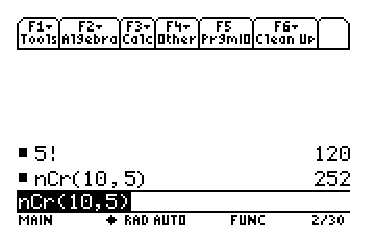
\includegraphics{eps/factorial}},{}]
Der Taschenrechner bietet die Funktionalität an, Fakultäten sowie
Binomialkoeffizienten einfach zu berechnen. Für Fakultäten kann dafür einfach
ein Ausrufezeichen hinter einen Ausdruck gesetzt werden. Dieses Ausrufezeichen
ist etwas versteckt, auf den TI-89 Modellen erscheint es mit der
Tastenkombination \keystroke{$\blacklozenge$}\keystroke{$\div$}, auf dem TI-92 Plus
und dem Voyage\texttrademark~200 nach der Betätigung von
\keystroke{2nd}\keystroke{W}. Binomialkoeffizienten können mit der Funktion
$\texttt{nCr(n,k)}$ berechnet werden. Diese Funktion kann, wie alle anderen
Funktionen, aus dem Funktionenkatalog ausgewählt werden. Dieser kann mit der
Taste \keystroke{CATALOG} aufgerufen werden; die Auswahl der Funktion erfolgt
mit Hilfe der Pfeiltasten, die Bestätigung mit der Taste \keystroke{ENTER}. In
der Abbildung wird die Fakultät $5!=120$ sowie der Binomialkoeffizient
${10\choose 5}=252$ ausgegeben.
\end{window}

\section{Summen}
\begin{window}[0,l,{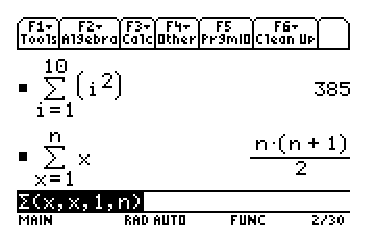
\includegraphics{eps/sum}},{}]
Oft ist es hilfreich, eine Summe der Form $ \sum_{i=a}^b s$
zu berechnen. Dies kann der Taschenrechner mit der Funktion \texttt{$\Sigma$()},
welche aus dem Katalog oder aus dem Menü \keystroke{F3} gewählt werden kann. In
der obigen Summe bezeichnet $i$ die Laufvariable, $a$ die untere und $b$
die obere Grenze und $s$ ist ein Summand, der typischerweise abhängig von $i$
ist. Die allgemeine Eingabe einer solchen Summe in den Taschenrechner lautet
folgendermassen: \texttt{$\Sigma$(s,i,a,b)}. Dabei können die einzelnen
Argumente frei gewählt werden (d.h. statt \texttt{i} kann als Laufvariable
ohne Weiteres auch \texttt{k} oder eine beliebige andere, nicht belegte Variable
gewählt werden), einzig die Reihenfolge muss beibehalten werden. Das erste
Argument steht für den Summanden, der aufsummiert wird, das zweite für die
Laufvariable und das dritte die untere bzw. obere Grenze. In der Abbildung
werden die Summen $\sum_{i=1}^{10} i^2$ und $\sum_{x=1}^n x$ berechnet.
\end{window}

\section{Gleichungen und Gleichungssysteme}
\begin{window}[0,l,{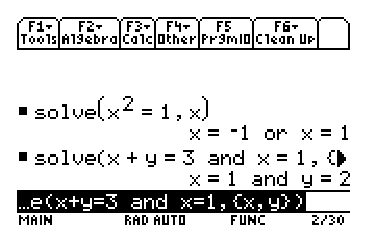
\includegraphics{eps/gls}},{}]
Gleichungen werden mit der Funktion \texttt{solve()} gelöst. Diese Funktion ist
im Katalog sowie im Menü \keystroke{F2} verfügbar. Die allgemeine Eingabe lautet
\texttt{solve(\textit{Gleichung},\textit{Unbekannte})}, um nach einer bestimmten
Unbekannten aufzulösen. In der Abbildung wird die Gleichung $x^2=1$ nach $x$
aufgelöst. Der Taschenrechner kann nicht nur einzelne Gleichungen, sondern ganze
Gleichungssysteme lösen. Dazu müssen die Gleichungen mit
\texttt{\textvisiblespace and\textvisiblespace} verknüpft und die Unbekannten
mit einer Liste (siehe Abschnitt \ref{list}) aufgezählt werden. Im Beispiel links wird das
Gleichungssystem
$$
\hspace{0.4\textwidth}\left|\begin{array}{lcc}
x+y&=&3\\
x&=&1\\
\end{array}\right|
$$
für $x_1$ und $x_2$ gelöst.
\end{window}

\section{Listen und Schätzer}\label{list}
In der Stochastik muss die selbe Rechenoperation oft mit einer ganzen Liste von
Zahlen durchgeführt werden. Man kann viel Zeit einsparen, indem man die
Rechenoperation gleichzeitig mit allen Zahlen durchführt. Dies kann man
erreichen, indem man alle Zahlen an der entsprechenden Position im Term in einer
Liste hinschreibt. Eine solche Liste besteht aus einer
kommagetrennten\footnote{Hier ist explizit die Komma-Taste \keystroke{,} gemeint
und nicht der Dezimalpunkt \keystroke{.}} Aufzählung von Zahlen, welche durch
geschweifte Klammern (\keystroke{\{} und \keystroke{\}}) abgeschlossen wird. Das
Prinzip soll anhand der folgenden Aufgabe erläutert werden:

\begin{quote}\textsl{Bei einem Würfel beträgt die Wahrscheinlichkeit, eine Sechs
zu werfen, \textbf{a)}$\frac{1}{6}$, \textbf{b)}$\frac{1}{7}$ oder
\textbf{c)}$\frac{1}{8}$. Wie gross ist die Wahrscheinlichkeit jeweils, in drei
Würfen drei Mal eine Sechs zu werfen?}\end{quote}

\begin{window}[0,l,{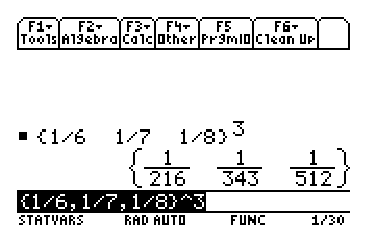
\includegraphics{eps/liste}},{}]
In diesem Beispiel müssen die Terme $\left(\frac{1}{6}\right)^3$,
$\left(\frac{1}{7}\right)^3$ und $\left(\frac{1}{8}\right)^3$ berechnet werden. Im
Taschenrechner können wir alle drei Rechnungen in einem Schritt durchführen,
indem wir die dritte Potenz der Liste \texttt{\{1/6,1/7,1/8\}} berechnen. Die
Reihenfolge der Listen-Elemente in der Ausgabe entspricht der Reihenfolge der
Eingabe.
\end{window}

\begin{window}[0,l,{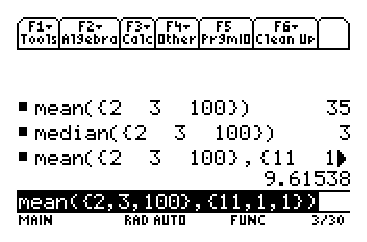
\includegraphics{eps/mean}},{}]
Listen eignen sich auch, um Schätzer zu berechnen. Wie in der Abbildung gezeigt kann
das arithmetische Mittel einer Liste mit der Funktion \texttt{mean()} ermittelt
werden. Der Median lässt sich mit \texttt{median()} analog bestimmen und für die
Varianz und die empirische Standardabweichung sind die Funktionen
\texttt{variance()} bzw. \texttt{stdDev()} vorgesehen. Mit Ausnahme von
\texttt{median()} erlauben all diese Funktionen ein zweites Argument, um eine
Gewichtung vorzunehmen: \texttt{mean(\textit{Werte},\textit{Gewichte})}.
\end{window}

\begin{window}[0,l,{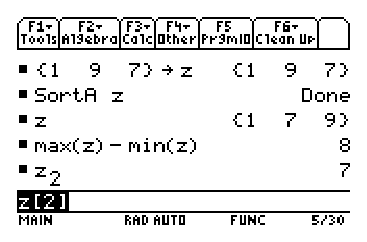
\includegraphics{eps/sort}},{}]
Die Bestimmung von exotischeren Schätzern ist etwas komplizierter. Eine grosse
Hilfe ist es jedoch das Sortieren einer Liste. Dazu muss diese im Vorfeld in
eine Variable gespeichert werden. Dies gelingt mit der Taste
\keystroke{STO$\blacktriangleright$} gefolgt von einer Variable. Es empfiehlt
sich, über solche vergebenen Variablen Buch zu führen und diese nicht als
symbolische Variablen in anderen Ausdrücken, insbesondere \texttt{solve()} und
\texttt{$\Sigma$()}, zu verwenden. Vergebene Variablen lassen sich mit
\keystroke{VAR-LINK} auflisten und entfernen. Die eigentliche Sortierung erfolgt mit Hilfe
von \texttt{SortA}. Quantile können anschliessend anhand der sortierten Liste
abgezählt werden. Die Variationsbreite kann mit Hilfe der Funktionen
\texttt{max()} und \texttt{min()} berechnet werden. Schliesslich lässt sich mit
\texttt{[\textit{Index}]} auf einzelne Listen-Elemente zugreifen; der Index beginnt bei 1.
\end{window}

\section{Integrale}
\begin{window}[0,l,{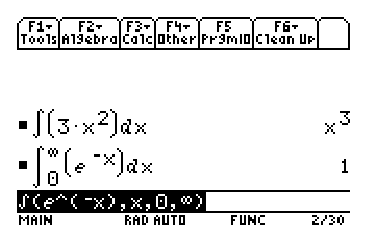
\includegraphics{eps/int}},{}]
Im Katalog und im Menü \texttt{F2} findet sich die Funktion \texttt{$\int$()},
mit der bestimmte und unbestimmte Integrale berechnet werden können.
Die allgemeine Eingabe lautet dabei für unbestimmte Integrale
\texttt{$\int$(\textit{Integrand}, \textit{Integrationsvariable})}, für bestimmte
Integrale müssen anschliessend noch untere und obere Grenze angegeben werden,
d.h.
\texttt{$\int$(\textit{Integrand},\textit{Integrationsvariable},\textit{unten},\textit{oben})}.

Die Abbildung zeigt die Berechnung des unbestimmten Integrals $\int 3x^2\mathrm{d}x$
sowie diejenige des bestimmten Integrals $\int_0^\infty\exp(-x)\mathrm{d}x$.
\end{window}

\section{Wobei-Operator}
\begin{window}[0,l,{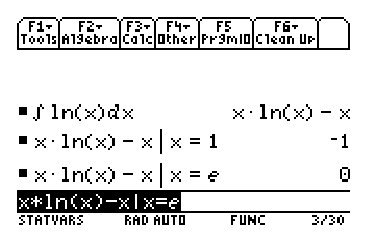
\includegraphics{eps/with}},{}]
Eine nützliche Taste ist der Wobei-Operator \keystroke{$|$}, der benutzt werden
kann, um einer Variable einen Wert zuzuweisen. Im Beispiel links wird zunächst
die Stammfunktion von $\ln(x)$ berechnet und anschliessend in diese Stammfunktion
nacheinander $x=1$ und $x=e$ eingesetzt. Nach dem Gleich-Zeichen können
Listen angegeben werden. Es ist auch möglich, zwei (verschiedene) Variablen
separat zu verwenden indem man sie mit \texttt{\textvisiblespace
and\textvisiblespace} verbindet: \texttt{x+y|x=1 and y=2}.
\end{window}



\section{Weitere Funktionen}
Die folgende Tabelle stellt einige weiteren Funktionen vor und erläutert, wie
diese aufgerufen werden müssen.

\begin{center}
{\scriptsize
\begin{longtable}{lllp{4.0cm}p{4.2cm}}\toprule
Eingabe & Ausgabe & Bedeutung & Beispiel \\\midrule
\texttt{cumSum(\textit{list})} & \textit{list} & Kumulative Summe &
\texttt{cumSum(\{1,2,3,4\})\begin{flushright}\{1,3,6,10\}\end{flushright}} \\
\midrule
\texttt{dim(\textit{list})} & \textit{int} & Anzahl Elemente &
\texttt{dim(\{3,6,1,$\pi$\})\begin{flushright}4\end{flushright}}  \\
\midrule
\texttt{$\Delta$list(\textit{list})} & \textit{list} & Differenzenfolge &
\texttt{$\Delta$list(\{1,3,6,10\})\begin{flushright}\{2,3,4\}\end{flushright}} \\
\midrule
\texttt{sum(\textit{list})} & \textit{exp} & Summe aller Elemente&
\texttt{sum(\{1,3,5\}) \begin{flushright}9\end{flushright}} \\
\bottomrule
\end{longtable}
}\end{center}

%\section{Symbolleiste}
%Die wichtigsten Befehle können in einer eigenen Symbolleiste zusammengefasst
%werden, um schnell verfügbar zu sein. Ein Beispiel wäre:
%
%\begin{description}
%\item[F1: Stoch] \texttt{nCr(,)}, \texttt{!}, \texttt{$\Sigma$(nCr(,)*p\^{}k*(1-p)\^{}(n-k),k,,n)}
%\item[F2: Stat] \texttt{mean()}, \texttt{variance()}, \texttt{stdDev()},
%\texttt{dim()}, \texttt{median()}, \texttt{sum()}
%\item[F3: PDF] \texttt{normPdf(,,,)}, \texttt{tPdf(,,)}, \texttt{Chi2Pdf(,)}, \texttt{FPdf(,,)}
%\item[F4: Inv] \texttt{invNorm(,,)}, \texttt{inv\_t(,)}, \texttt{invChi2(,)}, \texttt{invF(,,)}
%\item[F5: Ana] \texttt{d(,)}, \texttt{$\int$(,,)}, \texttt{$\Sigma$(,,,)},
%\end{description}

\cleardoublepage

\part{Stats/List Editor}
\section{Stats/List Editor: Erste Schritte}
\subsection{Installation}\label{installation}
Der \textit{Stats/List Editor} ist ein Programm für den Taschenrechner, der
die Durchführung vieler statistischer Methoden stark vereinfacht, indem es die
Berechnungen übernimmt. Diese Software ist allerdings nicht zwingend auf dem
Taschenrechner installiert. Sie kann aber kostenlos von der Texas Instruments
Webseite\footnote{\url{http://education.ti.com/educationportal/downloadcenter/SoftwareDetail.do?website=US&tabId=1&appId=189}}
heruntergeladen und mit einem Kabel auf den Taschenrechner überspielt
werden. Einfacher ist abber das Übertragen mit Hilfe eines anderen
Taschenrechners, auf dem das Programm bereits installiert ist. Unter Umständen
muss zusätzlich zur Software auch eine neuere Version des
Taschenrechner-Betriebssystems heruntergeladen und installiert werden.

\subsection{Starten}
Je nach Taschenrechner lässt sich der \textit{Stats/List Editor} auf
verschiedene Arten starten. Auf jeden Fall muss zunächst die Taste
\keystroke{APPS} gedrückt werden. Anschliessend erscheint entweder das
Applikationsmenü (linke Abbildung) oder die graphische Applikationsübersicht
(rechte Abbildung):

\begin{center}
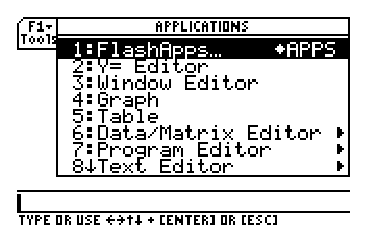
\includegraphics{eps/menuold}
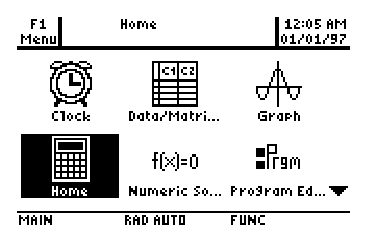
\includegraphics{eps/menunew}
\end{center}

\begin{window}[0,l,{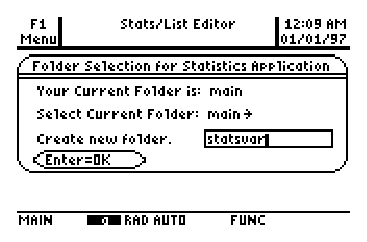
\includegraphics{eps/splash}},{}]
Im Applikationsmenü ist das Programm unter \texttt{1:Flash Apps} zu finden, in
der Applikationsübersicht lässt es sich einfach auswählen und starten. Nach dem
ersten Start muss ein Verzeichnis zur Speicherung der Variablen ausgewählt
oder erstellt werden. Es empfiehlt sich, ein neues Verzeichnis, z.B. wie in der
Abbildung \texttt{statsvar}, zu erstellen.
\end{window}

\begin{window}[0,l,{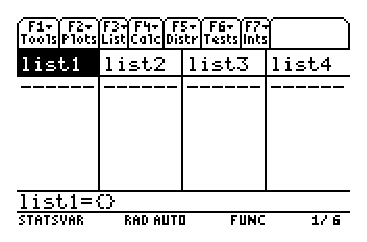
\includegraphics{eps/started}},{}]
Nach dem Definieren dieses Verzeichnisses und bei jedem weiteren Start erscheint
das Programm wie in der Abbildung gezeigt. Es lassen sich mit den
Funktionstasten \keystroke{F1} bis \keystroke{F7} Funktionen aufrufen, auf die
im Weiteren eingegangen wird. Im unteren Teil des Programmes lassen sich in den
Listen Daten eingeben, mit denen gearbeitet werden kann.
\end{window}

\section{Arbeiten mit dem Stats/List Editor}

\subsection{Operationen auf Listen}
\begin{window}[0,l,{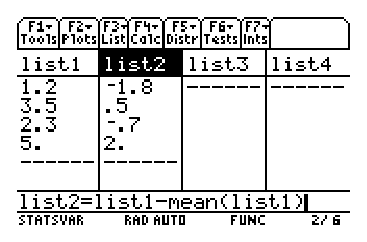
\includegraphics{eps/submean}},{}]
Um Daten in die Spalten der Tabelle einzutragen, muss der Cursor auf die
gestrichelte Linie (\texttt{-------}) plaziert werden. Nach der Betätigung von
\keystroke{ENTER} erscheint die eingegebene Zahl in der Zelle,
die gestrichelte Linie wandert um eine Zeile nach unten und erwartet direkt die
nächste Eingabe. Eine ganze Spalte kann gelöscht werden, indem der Cursor auf
die Spalten-Überschrift (z.B. \texttt{list1}) plaziert und anschliessend
\keystroke{CLEAR} und \keystroke{ENTER} gedrückt wird. Ausserdem kann man eine
Spalte mit einer Berechnung aus Zahlen von einer anderen Spalte befüllen. In der
Abbildung wird beispielsweise von jeder Zahl aus der Spalte \texttt{list1} der
Spaltenmittelwert abgezogen und das Resultat in der Spalte \texttt{list2}
eingetragen.
\end{window}

\begin{window}[0,l,{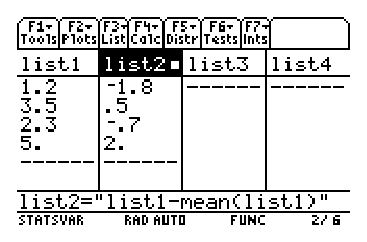
\includegraphics{eps/attachformula}},{}]
Allerdings wird bei diesem Vorgehen der neue Wert berechnet und direkt
eingetragen. Eine Änderung in der ersten Spalte -- z.B. die Korrektur eines
Tippfehlers -- führt daher nicht zu einer Korrektur der berechneten Werte. Diese
Funktion lässt sich aber durch Verwendung von Gänsefüsschen (\texttt{"}) 
wie in der Abbildung gezeigt herbeiführen. Eine so eingegebene \textit{Formel}
wird durch ein kleines schwarzes Quadrat im Spaltentitel markiert. Als
Alternative kann man für diese Funktion mit \texttt{4:Attach List Formula\ldots}
im Menü \keystroke{F3} ein Dialogfeld aufrufen.
\end{window}

\subsection{1-Var Stats}
\begin{window}[0,l,{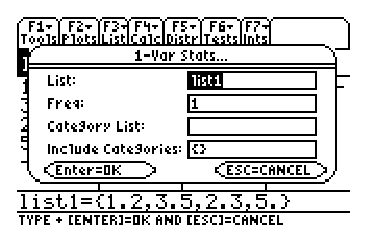
\includegraphics{eps/1vardialog}},{}]
Wenn von einem Datensatz gewisse Messgrössen wie Mittelwert oder
Standardabweichung gesucht sind, kann der \textit{Stats/List Editor} diese
Messgrössen in einer Tabelle ausgeben. Dazu muss der Datensatz zunächst in einer
Spalte eingegeben werden. Anschliessend kann die Funktion \texttt{1:1-Var Stats}
aus dem Menü \keystroke{F4} aufgerufen werden. Es erscheint ein Dialogfeld wie
in der Abbildung, in dem im Feld \texttt{List:} eingegeben werden muss, für
welche Spalte die Messgrössen berechnet werden sollen. Die anderen Felder dienen
der Gewichtung und der Eingabe von Klassen und können in den meisten Fällen
unverändert gelassen werden.
\end{window}

\begin{window}[0,l,{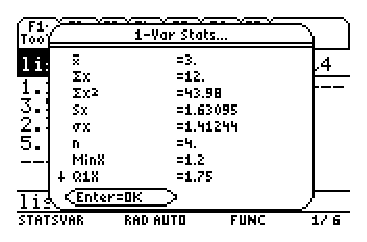
\includegraphics{eps/1vartable}},{}]
Nach der Betätigung von \keystroke{ENTER} erscheint die Tabelle mit den
Messgrössen. Die meisten Einträge sind selbsterklärend. Mit $\sum x^2$ ist
$\sum\left(x^2\right)$ und nicht etwa $\sum(x)^2$ gemeint (d.h. Summe der
Quadrate und nicht Quadrat der Summe). \texttt{Sx} ist die empirische
Standardabweichung mit Nenner $n-1$ und $\sigma x$ ist die Standardabweichung
der Grundgesamtheit mit Nenner $n$, hier ist also Vorsicht geboten. Ausserdem
werden Minimum, Maximum sowie erstes bis drittes Quartil angegeben.\footnote{Zur
Erinnerung: Der Median ist das zweite Quartil.}
\end{window}

\subsection{2-Var Stats}
Die Berechnung der Kenngrössen für zwei Datensätze gleichzeitig funktioniert analog
der Berechnung für eine Spalte, nur dass im Dialogfeld zwei Spalten angegeben
werden.


\subsection{Verteilungen}
\subsubsection{Dichteverteilungen und Wahrscheinlichkeitsfunktionen}
\begin{window}[0,l,{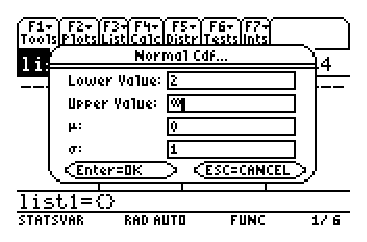
\includegraphics{eps/normdist}},{}]
Der  \textit{Stats/List Editor} enthält die gängigen Tabellen für diverse
Verteilungen. Diese lassen sich im Menü \keystroke{F5} abrufen. Die Abkürzungen
PDF bzw. CDF stehen für Dichtefunktion (\textit{probability distribution
function}) bzw. Wahrscheinlichkeitsfunktion (\textit{cumulative distribution
function}), wobei man im Dialogfeld für Wahrscheinlichkeitsfunktionen
Grenzen angeben kann. Sei beispielsweise $\varphi(x)=\mathcal{N}(0,1)$, so lässt sich 

\begin{eqnarray*}
\int_{2}^{\infty}\varphi(x)\mathrm{d}x=1-\int_{-\infty}^{2}\varphi(x)\mathrm{d}x=1-\Phi(2)\approx
0.05
 \end{eqnarray*}

mit \texttt{4:Normal Cdf...} wie in der Abbildung gezeigt berechnen.
\end{window}

Werte für $t$-, $F$-, $\chi^2$- und andere Verteilungen lassen sich analog
berechnen, wobei jeweils die Freiheitsgrade im Dialogfeld angegeben werden
müssen. Die folgende Abbildung zeigt die Berechnung eines p-Wertes einer ANOVA
mit $F=198.3$ mit 10 und 28 Freiheitsgraden.\footnote{Zur Erinnerung: Die Reihenfolge der
Freiheitsgrade spielt eine Rolle!}

\begin{center}
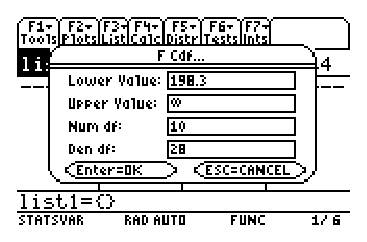
\includegraphics{eps/Fdist1}
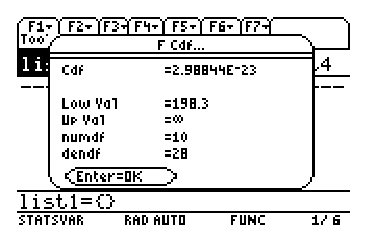
\includegraphics{eps/Fdist2}
\end{center}

\subsubsection{Quantil- bzw. Inversfunktionen}
Die Quantil-Funktionen für die Normal-, $t$-, $\chi^2$- und die F-Verteilung
sind im Menü \texttt{2:Inverse} unter \keystroke{F5} abrufbar. Die Abbildung
zeigt die Berechnung des kritischen Wertes für einen einseitigen t-Test mit
$\nu=19$ Freiheitsgraden auf einem Test-Level von 5\%.

\begin{center}
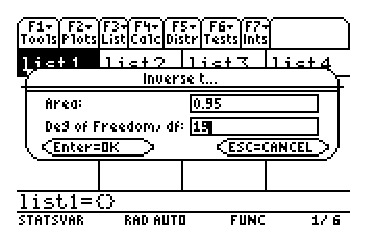
\includegraphics{eps/tdist1}
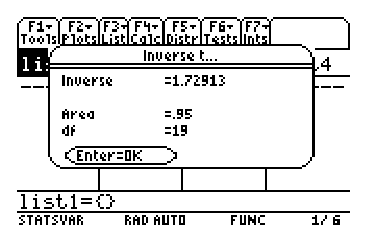
\includegraphics{eps/tdist2}
\end{center}

Der kritische Wert ist also etwa 1.73.

\subsection{T-Tests}
Der \textit{Stats/List Editor} ist eine grosse Hilfe beim Durchführen von Tests.
Alle unterstützten Tests sind im Menü \keystroke{F6} abrufbar.
\subsubsection{One Sample T-Test}
\begin{window}[0,l,{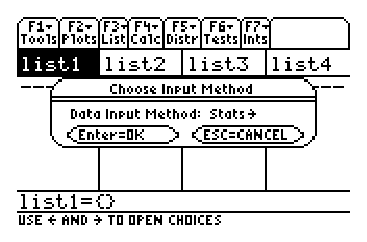
\includegraphics{eps/tchoose}},{}]
Der One Sample T-Test kann im Menü \keystroke{F6} mit \texttt{2:T-Test\ldots}
aufgerufen auf zwei verschiedene Arten durchgeführt werden. Entweder wurden der
Stichproben-Mittelwert \texttt{$\bar{x}$} und die empirische Standardabweichung
\texttt{Sx} schon berechnet oder sind gegeben, oder sie können direkt aus einer
Liste berechnet werden. Im ersten Fall ist im Dialogfeld in der Abbildung
\texttt{Stats} zu wählen, im zweiten Fall \texttt{Data}.
\end{window}

Je nach Auswahl erscheinen danach zwei unterschiedliche Dialogfelder, in denen
die statistischen Masse oder die Liste mit den Daten eingegeben werden können:

\begin{center}
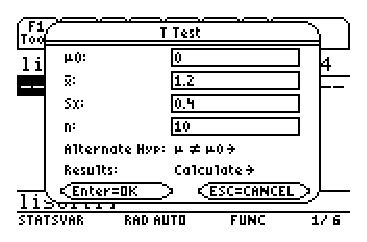
\includegraphics{eps/tstats.eps}
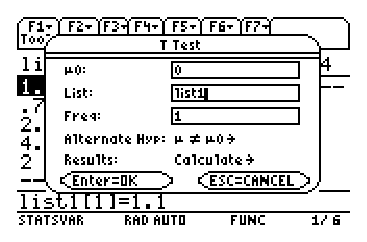
\includegraphics{eps/tdata.eps}
\end{center}

Ausserdem müssen die Stichprobengrösse $n$ sowie die Prüfgrösse $\mu_0$
eingegeben sowie die \textbf{Alternativ}-Hypothese gewählt werden.

\begin{window}[0,l,{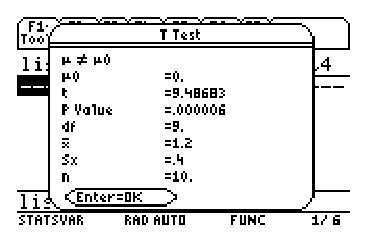
\includegraphics{eps/tresult}},{}]
Nach der Bestätigung mit \keystroke{ENTER} erscheinen die Resultate des Tests
wie in der Abbildung gezeigt. Insbesondere wird der berechnete T-Wert unter
\texttt{t} sowie der daraus resultierende p-Wert unter \texttt{p Value}
aufgeführt. Zudem kann man die Prüfgrösse $\mu_0$, die Freiheitsgrade
\texttt{df}, den Stichproben-Mittelwert $\bar{x}$, die empirische
Standardabweichung \texttt{Sx} sowie die Stichprobengrösse $n$ ablesen.
\end{window}

\subsubsection{Two Sample T-Test}
Der Two Sample T-Test ist im Menü \keystroke{F6} unter
\texttt{4:2-SampTTest\ldots} zu finden. Die Eingabe funktioniert analog
derjenigen beim One Sample T-Test. Ausserdem kann unter \texttt{Pooled} gewählt
werden, ob die Varianzen gepoolt werden oder nicht. Der T-Test verlangt als
Voraussetzung gleiche Varianzen, welche in der Teststatistik dann gepoolt
werden. Falls die Varianzen nicht gleich sind, kann man dies korrigieren, statt
die Varianzen einfach zu poolen. In der Vorlesung wurde aber nur der Fall mit
gepoolten Varianzen vorgestellt, daher kann dort die Einstellung \texttt{YES}
gewählt werden.

\subsubsection{Paired T-Test}
%\begin{window}[0,l,{\includegraphics{eps/tpaired}},{}]
Der Paired T-Test (T-Test mit gepaarten Daten) ist eigentlich ein One Sample
T-Test, der mit den Differenzen der gepaarten Daten berechnet wird. Deshalb kann
man zur Durchführung einfach einen One Sample T-Test machen und mit den
Differenzen (z.B. \texttt{list2-list1}) arbeiten.
%\end{window}


\subsection{Konfidenzintervalle}
\begin{window}[0,l,{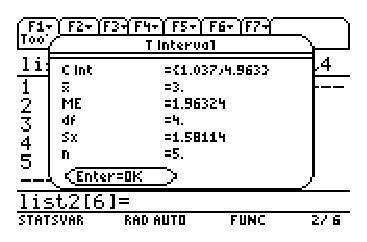
\includegraphics{eps/ki2}},{}]
Im Menü \keystroke{F7} lassen sich Dialogfelder aufrufen, mit denen man
Konfidenzintervalle berechnen lassen kann. Je nach Aufgabenstellung wählt man
\texttt{2:TInterval\ldots} für den Einstichproben-Fall und
\texttt{4:2SampleTInt\ldots} für den Zweistichproben-Fall. Die Daten lassen sich
dabei genau wie bei den T-Tests eingeben -- bei gegebenen Schätzungen mit
\texttt{Stats}, oder aber mit \texttt{Data}, falls die Schätzungen erst noch
berechnet werden müssen. Ausserdem lässt sich mit \texttt{C Level} das
Konfidenzniveau (üblicherweise 95\%=0.95), angeben.
\end{window}

\begin{window}[0,l,{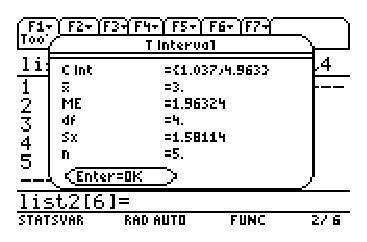
\includegraphics{eps/ki2}},{}]
Nach der Bestätigung mit der Taste \keystroke{ENTER} erscheint ein Dialogfeld,
in dem das Konfidenzintervall \texttt{C Int}, der Stichprobenmittelwert
$\bar{x}$, die Intervallbreite (Margin of Errors) \texttt{ME} sowie empirische
Standardabweichung \texttt{Sx} und Stichprobengrösse $n$ abgelesen werden
können. Das Konfidenzintervall erscheint in der Notation
\texttt{\{\textit{untere Grenze},\textit{obere Grenze}\}}, im Beispiel handelt
es sich um das Intervall $[1.037, 4.963]$.
\end{window}


\subsection{Einfache ANOVA}
\begin{window}[0,l,{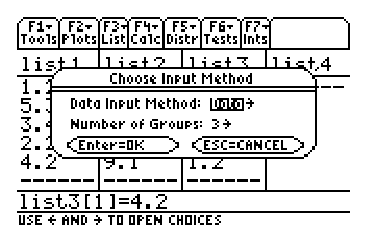
\includegraphics{eps/anova1}},{}]
Um eine ANOVA durchzuführen, müssen die Daten zunächst in die Tabelle eingegeben
werden. Theoretisch können auch hier analog zu den T-Tests und den
Konfidenzintervallen mit \texttt{Stats} gegebenen Kenndaten verwendet werden,
worauf hier aber nicht weiter eingegangen wird. Nach der Eingabe der Daten kann
im Menü \keystroke{F6} \texttt{C:ANOVA} aufgerufen werden. Es erscheint ein
Dialogfeld, indem die Anzahl Gruppen eingegeben werden. Da die Daten in der
Tabelle vorliegen, soll ferner als \texttt{Data Input Method} die Option
\texttt{Data} gewählt werden.
\end{window}

\begin{window}[0,l,{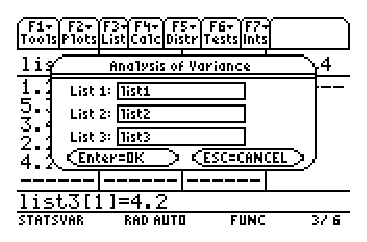
\includegraphics{eps/anova2}},{}]
Im nächsten Dialogfeld müss spezifiziert werden, in welchen Spalten die Daten
eingegeben wurden. Falls die Daten bei drei Gruppen in den ersten drei Spalten
eingetippt wurden, so sind hier die Namen dieser ersten drei Spalten anzugeben.
Üblicherweise handelt es sich dabei einfach um \texttt{list1}, \texttt{list2}
und \texttt{list3}. (Der Name der Spalte ist im Spaltentitel jeweils angegeben).
\end{window}

\begin{window}[0,l,{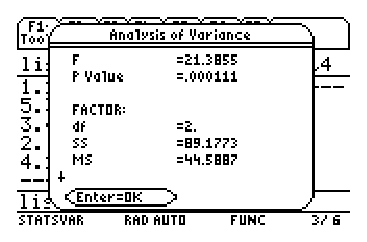
\includegraphics{eps/anova3}},{}]
Nach der Bestätigung mit der Taste \keystroke{ENTER} erscheint ein Dialogfeld
mit den Resultaten. Zuoberst erscheinen F- und p-Werte zu den gegebenen
Daten. Anschliessend lassen sich die erste Zeile der ANOVA Tabelle
(\texttt{FACTOR} bzw. \textit{between}-Werte) und die
zweite Zeile (\texttt{ERROR} bzw. \textit{within}-Werte) der ANOVA-Tabelle ablesen. Angegeben werden
jeweils die Freiheitsgrade (\texttt{df}), die Quadratsumme (Sum of Squares,
\texttt{SS}), sowie der Quotient aus Quadratsumme und Freiheitsgraden (Mean
Square, \texttt{MS}).
\end{window}

\subsection{Einfache Lineare Regression}
\begin{window}[0,l,{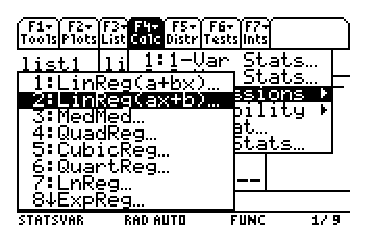
\includegraphics{eps/lrmenu}},{}]
Eine lineare Regression lässt sich nach der Eingabe der $x$- und $y$-Koordinaten
aus dem Menü \keystroke{F4} mit \texttt{Regressions$\RHD$}
berechnen. Dabei stehen zwei Formen zu Verfügung, nämlich
\texttt{1:LinReg(a+bx)} sowie \texttt{2:LinReg(ax+b)}. Der Unterschied zwischen
diesen beiden Formen ist lediglich die Bezeichnung der Variablen. Im ersten Fall
ist $a$ der y-Achsenabschnitt und $b$ die Steigung, im zweiten Fall ist es
umgekehrt. Üblicherweise wird die zweite Notation verwendet, deshalb ist es
angebracht, \texttt{2:LinReg(ax+b)} zu wählen.
\end{window}

\begin{window}[0,l,{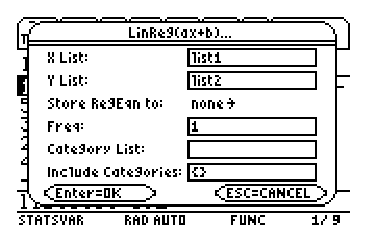
\includegraphics{eps/lrdiag}},{}]
Im nächsten Dialogfeld muss definiert werden, in welchen Spalten der Tabelle die
$x$- und $y$-Koordinaten eingegeben wurden. Ausserdem besteht die Möglichkeit,
die Regressionsfunktion bzw. Geradengleichung mit \texttt{Store RegEqn to:} zu
speichern, um sie danach zu plotten. Die weiteren Felder dienen zur Einführung
von Klassen und Häufigkeiten und werden an dieser Stelle nicht behandelt.
\end{window}

\begin{window}[0,l,{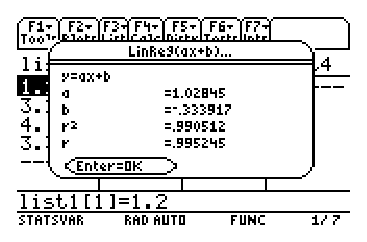
\includegraphics{eps/lrresult}},{}]
Nach der Bestätigung mit der Taste \keystroke{ENTER} erscheint ein Dialogfeld
mit den Resultaten. Es werden Schätzungen für den y-Achsenabschnitt und die
Steigung angegeben. Ausserdem erscheinen das Bestimmtheitsmass
(Determinationskoeffizient) $r^2$ sowie der Korrelationskoeffizient $r$. (Siehe
Vorlesungsskript, Abschnitt 10.2.4, \textit{Korrelation}, p. 173f.)
\end{window}

\begin{window}[0,l,{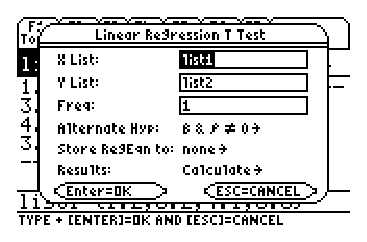
\includegraphics{eps/lrtest1}},{}]
Schlussendlich kann man noch Tests zur Geradensteigung machen. Will man die
Nullhypothese $\mathcal{H}_0: \beta_1=0$ (wahre Steigung ist 0) testen, so kann
man dies im Menü \keystroke{F6} unter \texttt{A:LinRegTTest\ldots} tun. Im
Dialogfeld sind wie üblich die Spalten mit den Daten anzugeben. Die
Alternativhypothese \texttt{$\beta$ \& $\rho\ne 0$} entspricht dabei der
gegebenen Fragestellung. (Siehe Vorlesungsskript, Abschnitt 10.2.1.4,
\textit{Testen ob $\beta_1=0$}, p. 262f.).
\end{window}

\begin{window}[0,l,{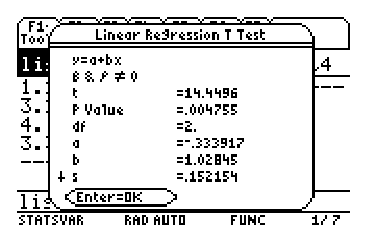
\includegraphics{eps/lrtest2}},{}]
Das Dialogfeld mit den Ergebnissen präsentiert wie üblich einen t- und einen
p-Wert. Ausserdem lassen sich die Schätzungen für die Parameter auch hier
zusammen mit weiteren Kenngrössen ablesen. Beim Test auf die wahre Steigung einer linearen Regression ist
allerdings nur das Modell $y=a+bx$ auswählbar, $a$ ist also immer der
y-Achsenabschnitt und $b$ immer die Steigung. 
\end{window}

\section{$\chi^2$-Tests}
\subsection{Goodness Of Fit}
Mit dem $\chi^2$-Test ist es möglich, zu testen, ob eine Stichprobe einer
bestimmten Verteilung folgt ($=\mathcal{H}_0$). Dazu ist die Stichprobe in eine
erste Spalte und die erwarteten Werte in eine zweite Spalte einzutragen.
Anschliessend kann aus dem Menü \keystroke{F6} der Punkt \texttt{7:Chi2 GOF}
aufgerufen werden. Das erscheinende Dialogfeld erwartet die Spalten mit der
Stichprobe (\texttt{Observed List}), die Spalte mit den erwarteten Werten
(\texttt{Expected List}) sowie die Anzahl Freiheitsgrade. Nach der Bestätigung
mit \keystroke{ENTER} wird der $\chi^2$-Wert sowie ein p-Wert zurückgegeben.

\subsection{Test auf Unabhängigkeit}
Der $\chi^2$-Test kann auch verwendet werden, um auf Unabhängigkeit zu testen.
Dazu ist die Kontingenztafel aufzustellen, mit deren Hilfe bei einer manuellen
Auswertung die Randsummen berechnet würden. Als Beispiel soll folgende
theoretische Kontingenztafel mit 4 Felder dienen:

\begin{center}\begin{tabular}{l|cc|l}
 & Krank & Gesund & Randsumme\\\toprule
Treatment & $x_{kt}$ & $x_{gt}$ & $x_{kt}+x_{gt}$\\
Control   & $x_{kc} $ & $x_{gc}$ & $x_{kc}+x_{gc}$\\\midrule
Randsumme & $x_{kt}+x_{kc}$ & $x_{gt}+x_{gc}$ & $x_{kt}+x_{gt}+x_{kc}+x_{gc}$\\\bottomrule
\end{tabular}\end{center}

Die Kontingenztafel ist etwas umständlich in den Taschenrechner einzugeben: Die
Zellen müssen mit einem Komma (Taste \keystroke{,}) getrennt werden, die Zeilen
mit eckigen Klammern (\keystroke{[} und \keystroke{]}). Die ganze Tabelle muss in
ein weiteres Paar eckige Klammern verpackt werden, so dass für die obige Tabelle
folgendes eingegeben wird: \texttt{[[$x_{kt}$,$x_{gt}$][$x_{kc}$,$x_{gc}$]]}

\end{document}
